\chapter{État de l'art}
\label{chap:Etat de l'art}

\section{Architecture d'Entreprise}

\subsection{Terminologie}

\textbf{Système d'Information (SI)}

Selon Robert Reix, le SI est "~un ensemble organisé de ressources : matériel, 
logiciel, personnel, données, procédures permettant d'acquérir, de traiter, de 
stocker des informations (sous forme de donnée, textes, images, sons, etc.) dans 
et entre des organisations.~"

Nous adoptons cette définition car elle a l'avantage de ne pas réduire le SI 
d'une organisation à son système informatique. Ce dernier est constitué de 
l'ensemble du patrimoine matériel (hardware) et applicatif (software) de la dite 
organisation et a pour objectif d'automatiser le traitement de l'information. Nous adoptons l'acronyme IT (\textit{Information Technologie}) pour le différencier du SI.

On suppose souvent que tout les SI sont totalement informatisés et c'est une des raisons qui amène à confondre SI et IT. Cependant, le SI comprend le système non seulement le informatique mais aussi des ressources humaines (partenaires, personnel, etc.) et immatérielles (procédures de gestion, savoir-faire métier, etc.).



\textbf{Architecture d'Entreprise  (AE)}

Selon Scott Bernard \cite{bernard2012introduction}, une entreprise est une 
organisation ou une sous-partie d'une organisation qui poursuit des objectifs 
communs, en s'appuyant sur les mêmes processus et en utilisant les mêmes 
ressources. Une entreprise peut être publique ou privée, avoir ou pas un but 
lucratif. 

Dans ce contexte, l'Architecture d'Entreprise est une discipline qui a pour 
vocation de décrire une telle organisation en offrant une vue générale et 
homogène de son métier, de son patrimoine applicatif et de infrastructure 
technique ainsi que leur évolution pour en faciliter l'analyse par biais d'un 
ensemble cohérents de principes, méthodes et modèles 
\cite{lankhorst2009enterprise}.

Par analogie avec l'architecture de bâtiment, construire une maison en procédant 
chambre par chambre sans plan d'architecture général peut mener à un résultat 
peu probant. Il en est de même pour le développement d'une organisation sans une 
architecture globale de référence, entrainant ainsi une duplication des 
ressources et donc un manque d'efficacité \cite{bernard2012introduction}.

Dans la littérature, il existe une multitude de définitions de l'AE émanant du 
monde académique mais aussi industriel. Néanmoins, aucune définition n'a été 
universellement adoptée \cite{mentz2012comparison} 
\cite{ranganathan2005enterprise}. Ce fait est certainement du à la nature 
intrinsèque de l'AE. En effet, cette dernière est régie par un ensemble de 
préceptes et de bonnes pratiques que chacun reste libre d'adapter à son propre 
besoin. C'est ce qui a amené Dankova à classifier les définitions existantes 
selon l'aspect sur lequel leurs auteurs décident de mettre l'accent. Il en 
ressort quatre catégories de définition : 
\begin{itemize}
\item Planification et conception

L'AE représente un plan descriptif de la structure d'une organisation avec ses 
différents composants et les relations entre ces composants. La but de ce plan 
étant de trouver le moyen le plus efficace pour que l'entreprise  son objectif.
\item Planification et conception

L'AE est conçue comme un ensemble de principes, de règles et de modèles que doit 
respecter l'implémentation de l'entreprise ne partant du métier jusqu'à 
l'infrastructure technique.
\item ICT

\textcolor{red}{to do}
\item Métier

\textcolor{red}{to do}
\end{itemize}


Cependant, cette classification révèle que le terme AE peut prêter à confusion 
car il est à la fois utilisé pour désigner :
\begin{itemize}
\item l'activité de conception d'une architecture i.e. la description des 
éléments composant l'organisation en question et leurs relations mais aussi 
\item l'ensemble des artefacts résultant de cette activité.
\end{itemize}

Pour éviter toute confusion, nous désignons l'activité de conception par le 
terme Architecture d'Entreprise et résultat de cette activité comme 
l'architecture de l'entreprise.

\textcolor{red}{Cette partie est encore un sacré chantier...}


\subsection{De l'architecture IT vers l'Architecture d'Entreprise}

L'origine de l'EA\footnote{D'après Scott Bernard \cite{bernard2012introduction}, le terme Architecture d'Entreprise a fait sa première apparition dans le livre de Steven Spewak intitulé "Enterprise Archietcture Planning : developing a blueprint for data, applications and technology" \cite{spewak1993enterprise}.} remonte au travaux de Zachman qui est souvent considéré comme le père de l'AE. Dans ces travaux précurseurs, il propose un cadre d'architecture pour l'IT \cite{zachman1987framework}.

Ainsi, l'Architecture d'Entreprise (AE) a initialement été conçue pour optimiser la 
gestion du patrimoine applicatif et de l'infrastructure technique d'une 
entreprise \cite{kappelman2008enterprise}. À ses débuts, l'AE se 
focalise sur les artefacts liés aux technologies de l'information comme les 
plateformes et les processus applicatifs, les équipements informatiques, les bases de données et les réseaux de télécommunications dans l'optique d'une gestion plus efficace et d'un meilleur retour sur investissement 
\cite{winter2006essential}. 

Cependant, le rôle de plus en plus prégnants de l'IT et son impact sur le c\oe{}ur de métier des organisations ainsi que l'accroissement de sa complexité \cite{ranganathan2005enterprise} ont fait de l'architecture de l'IT d'une entreprise une problématique inhérente à l'architecture de l'ensemble de l'entreprise. Ainsi, l'AE a commencé à intégrer des aspects métier tels que les objectifs de l'organisation, les processus métier, les indicateurs de performances \cite{winter2006essential}. En intégrant ainsi des problématiques métier, L'AE ne relève plus de l'architecture IT mais de l'architecture du SI dans son ensemble.

Pour Scott Bernard, l'AE doit même aller plus loin en intégrant les aspects concernant la stratégie de l'entreprise \cite{bernard2012introduction}. L'AE devient ainsi un instrument pour profiter pleinement de l'ensemble des ressources de l'entreprise (métier, IT, humaines, etc.). Pour Schott Bernand, le terme "~entreprise~" implique donc une vue stratégique de haut niveau de l'organisation dans son ensemble. Quand au terme "~architecture~", il implique la mise en place d'une cadre structuré pour l'analyse, le planning, et le développement de toutes les ressources dont dispose cette organisation.  

  




L'Architecture d'Entreprise (AE) est un moyen efficace pour capturer les 
composants d'une entreprise dans ses états courants et désirés.  

Une modélisation appropriée d'une telle architecture reflète donc les besoins 
des acteurs (expert du domaine métier, architecte fonctionnel, architecte 
technique, etc.) en explicitant les informations manipulées.  
\\Étant donnée la complexité des SI actuels, en particulier ceux des Smart 
Grids, et la multitude des acteurs concernés, une vision monolithique est 
inappropriée à la construction de SI évolutifs et adaptés aux différents 
acteurs.
\\Plusieurs cadres d'architecture adoptent une approche par points de vue. Un 
point de vue formalise la perspective d'un acteur particulier du SI. Une vue est 
conforme à ce point de vue. C'est le cas de RM-ODP \cite{raymond1995reference}, 
de TOGAF \footnote{The Open Group Architecture Framework} 
\footnote{www.opengroup.fr/togaf}, de la méthode « 4+1 » de Kruchten 
\cite{kruchten19954+} ainsi que de la norme ISO/IEC/IEEE 
42010\footnote{http://www.iso-architecture.org/}. Le SGAM\footnote{Smart Grid 
Archietcture Model} \cite{uslar2012standardization} adresse l'architecture du 
Smart Grid en englobant les trois domaines : SI, réseau électrique et réseau de 
télécommunication. 
\\En outre, ces frameworks organisent hiérarchiquement les différentes vues en 
appliquant \emph{« IT follows business »} comme principe : commencer par le 
point de vue métier et le dériver progressivement jusqu'à l'infrastructure 
technique déployée en passant par les fonctions et les applications 
\cite{winter2006essential}. 
Souvent, ces cadres d'architecture distinguent quatre points de vue principaux~:
\begin{description}
\item[Point de vue métier]  : ce point de vue reflète la vision métier. On y 
retrouve les objectifs métier de l'entreprise, les processus, ainsi que les 
acteurs~;
\item[Point de vue fonctionnel] : ce point de vue organise le SI en blocs 
fonctionnels de manière à garantir son évolutivité tout en répondant aux besoins 
métier de l'entreprise. A l'échelle du SI d'une entreprise, cette structuration 
devient vite complexe à cause du caractère étendu et transverse des processus 
métier impactés~;
\item[Point de vue applicatif] : ce point de vue structure le SI en blocs 
applicatifs, chacun implantant un ou plusieurs blocs fonctionnels~;
\item[Point de vue technique] : ce point de vue correspond à l'infrastructure 
technique du SI (matériel informatique et réseaux télécom).
\end{description}




\section{Ingénierie Dirigée par les Modèles}

L'Ingénierie Dirigée par les Modèles (IDM) est née du constat que le paradigme 
du « tout est objet », prôné dans les années 1980, a atteint ses limites avec ce 
début de siècle \cite{greenfield2004software}. En effet, face à la croissance de 
la complexité des systèmes logiciels, au coût de la main d'œuvre et de 
maintenance, une approche centrée sur le code, jugé alors seul représentant 
fiable du système, suscitait de moins en moins l'adhésion des industriels et du 
milieu académique. 

Partant de ce constat, l'Object Management Group (OMG) a proposé en novembre 
2000, l'approche MDA (Model Driven Architecture) qui s'inscrit dans le cadre 
plus général de l'IDM et se réalise autour d'un certain nombre de standards tels 
qu'UML, MOF, XML, QVT, etc. Le monde de la recherche s'y est aussitôt intéressé 
pour dégager les principes fondamentaux de l'IDM 
\cite{bezivin2001towards}\cite{kent2002model} \cite{de2002using} et déjouer le 
piège des définitions parfois trop floues qui prêtent à confusion entre les 
concepts liés aux paradigmes d'objet et de modèle \cite{bezivin2004search}. Par 
ailleurs, des industriels comme IBM \cite{booch2004mda} et Microsoft 
\cite{greenfield2004software} ont aussi rendu publiques leur vision de l'IDM. 
Ainsi, l'IDM prend son origine dans la convergence de toutes ces visions et des 
avancées techniques de chacun.

L'originalité de l'IDM ne réside pas dans le recours systématique aux modèles 
dans le développement logiciel comme le laisserait entendre sa terminologie  
\cite{bezivin2004rapport}. Plusieurs méthodes de modélisation telles que Merise 
ou SSADM préconisent aussi l'utilisation de modèles dont le rôle s'achève aux 
phases amont du développement logiciel : l'analyse et la conception. Les modèles 
servent alors à faciliter la communication et compréhension entre les différents 
acteurs mais n'interviennent pas dans la phase de production, de maintien et 
d'évolution. Nous parlons dans ce cas de modèles « contemplatifs ». 

L'IDM a pour objectif de rendre les modèles « productifs » sur tout le cycle de 
vie du système et à tout niveau d'abstraction. Pour y parvenir, les modèles 
doivent être décrits formellement pour être interprétés et exécutés par une 
machine. Dès lors, ces modèles permettent d'industrialiser la production 
logicielle, jusque-là centrée sur le code produit par l'informaticien 
\cite{bezivin2005unification}.

En mettant à profit des disciplines comme la modélisation par objets, 
l'ingénierie des langages, la compilation de langages, les méthodes formelles, 
la programmation par composants, etc., l'IDM offre un cadre intégrateur reposant 
sur quelques concepts fondamentaux : la notion de modèle et la relation 
\textit{ReprésentationDe}, la notion de métamodèle et la relation 
\textit{ConformeÀ}.

\subsection{Concepts et relations de l'IDM}
\subsubsection{Modèle et ReprésentationDe}
La notion de modèle est centrale dans l'IDM car, comme nous venons de voir, 
l'enjeu de cette approche est de rendre les modèles productifs sur tout le cycle 
de vie du système. Il n'existe pas de définition universelle de la notion de 
modèle. En nous appuyant sur les définitions données dans les travaux 
\cite{minsky1967computation} \cite{bezivin2001towards} et 
\cite{seidewitz2003models}, nous adoptons la définition suivante du terme modèle 
:

\begin{theorem}
Un modèle est une abstraction d'un système, selon le bon point de vue, qui 
permet de répondre à des questions prédéfinies sur ce système en lieu et place 
de celui-ci.
\end{theorem}

De cette définition découle la première relation fondamentale de l'IDM qui lie 
le modèle et le système qu'il représente. Celle-ci est nommée 
\textit{ReprésentationDe} et notée $(\mu)$. Bien que la relation 
\textit{ReprésentationDe} ne soit pas nouvelle dans l'ingénierie logicielle 
(Merise, UML), l'IDM a permis d'en définir les contours \cite{atkinson2003model} 
\cite{seidewitz2003models} \cite{bezivin2004search}.

\begin{figure}[!htbp]
 \begin{center}
  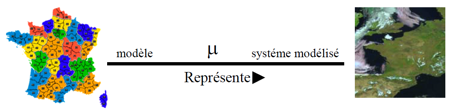
\includegraphics[width=1\textwidth]{Chapitre1/favresystememodele.png}
 \end{center}
 \caption{Relation entre système et modèle \protect\cite{favre2006ingenierie}}
 \label{fig:systemModele}
\end{figure}

Cette définition n'est pas restreinte à l'informatique et pourrait s'appliquer à 
n'importe quel système. 
La figure~\ref{fig:systemModele} reprend l'exemple connu de la cartographie où 
une carte géographique joue le rôle de modèle pour une région donnée jouant 
alors le rôle de système modélisé. 

L'intérêt de l'IDM est de produire des modèles exploitables informatiquement. 
Ceci n'est possible que si ces modèles sont décrits par des langages formels. Il 
devient alors important de bien définir ces langages à l'aide de métamodèles

\subsubsection{Métamodèle et ConformeÀ}
L'originalité de l'IDM ne réside pas dans la relation ReprésentationDe qui 
trouve plutôt son origine dans les méthodes de modélisation telles que Merise ou 
SSADM. L'apport de l'IDM est dans l'utilisation systématique de métamodèles pour 
la description des langages de modélisation. 

Il existe plusieurs définitions de la notion de métamodèle dans la littérature. 
Cependant la définition suivante est communément admise 
\cite{bezivin2004rapport}.

\begin{theorem}
Un métamodèle est un modèle du langage de modélisation qui sert à exprimer les 
modèles.
\end{theorem}
Une autre définition courante mais erronée de la notion de métamodèle suppose 
qu'un métamodèle est un modèle d'un modèle. La figure~\ref{fig:modelofmodel} 
reprend l'exemple de la cartographie évoquée plus haut. Nous appliquons 
récursivement la relation \textit{ReprésentationDe} $(\mu)$ au territoire 
français. Ici une carte de la France joue le rôle de modèle du territoire 
français et un fichier XML joue le rôle de modèle de la carte. Dans ce contre 
exemple, le fichier XML n'est pas un métamodèle de la France. Un métamodèle 
n'est donc pas un modèle d'un modèle.

\begin{figure}[!htbp]
 \begin{center}
  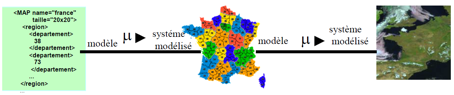
\includegraphics[width=1\textwidth]{Chapitre1/modelofmodel.png}
 \end{center}
 \caption{Modèle de modèle selon l'exemple de la cartographie 
\protect\cite{favre2006ingenierie}}
 \label{fig:modelofmodel}
\end{figure}

Par ailleurs, le concept de métamodèle induit la deuxième relation fondamentale 
de l'IDM liant un modèle à son métamodèle. Cette relation est nommée 
\textit{ConformeÀ} et notée $\chi$ \cite{bezivin2004search} 
\cite{favre2004towards}. La figure \ref{fig:carteFavre} reprend l'exemple de la 
cartographie où la légende de la carte joue le rôle de métamodèle ($\chi$) pour 
une carte de la France. En effet, pour être lisible, la carte doit être conforme 
à la légende.

\begin{figure}[!htbp]
 \begin{center}
  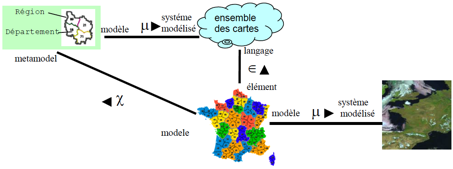
\includegraphics[width=1\textwidth]{Chapitre1/cartecompleteIDM.png}
 \end{center}
 \caption{Relations entre système, modèles, métamodèle et langage de 
modélisation \protect\cite{favre2006ingenierie}}
 \label{fig:carteFavre}
\end{figure}

\subsection{Transformation de modèle}
Dans la partie précédente, nous avons introduit les concepts fondamentaux de 
l'IDM que représentent la notion de modèle et la relation 
\textit{ReprésentationDe} ainsi que la notion de métamodèle et la relation 
\textit{ConformeÀ}. Comme expliqué, la préoccupation majeure de l'IDM est de 
rendre les modèles opérationnels sur tout le cycle de vie des systèmes 
logiciels, depuis l'analyse et la conception jusqu'à la maintenance et 
l'évolution. Ainsi, la transformation de modèle se retrouve au cœur de l'IDM car 
c'est à travers elle que se fait l'automatisation des traitements apportés aux 
modèles. Nous allons d'abord donner une définition de la notion de 
transformation de modèle puis en présenter les types et les usages.

\subsubsection{Définition de la transformation de modèle}
L'OMG définit une transformation de modèle comme «~le processus consistant à 
convertir un modèle en un autre modèle d'un même système~» \cite{omg2011meta}. 

\cite{kleppe2003mda} proposent une définition moins générique en insistant sur 
l'aspect automatique de ce processus, ainsi, «~une transformation de modèle 
consiste en la génération automatique d'un modèle source en un modèle cible, 
selon une description établie de cette transformation~». Cette définition 
implique aussi qu'une transformation est décrite à un plus haut niveau 
d'abstraction : au niveau d'un métamodèle auquel elle doit se conformer. 

\cite{mens2006taxonomy} étendent cette définition en considérant qu'une 
transformation est une opération qui peut avoir en entrée un ou plusieurs 
modèles source et en sortie un ou plusieurs modèles cible~: 

\begin{theorem}
Une transformation génère automatiquement un ou plusieurs modèles cible à partir 
d'un ou plusieurs modèles source, selon une description établie de la 
transformation. 
\end{theorem}

C'est cette dernière définition que nous allons adopter dans ce document. Par 
ailleurs, notons que, si les métamodèles source et cible sont différents, la 
transformation est dite exogène. Si les métamodèles source et cible 
correspondent au même métamodèle, la transformation est dite endogène. Ces 
termes ont été introduits par \cite{mens2006taxonomy}.

\subsubsection{Composants d'une transformation de modèle} 
La figure \ref{fig:composantTransfo} illustre les composants d'une 
transformation de modèle~:~les modèles source, les modèles cible, la définition 
de la transformation et le moteur qui va opérer la transformation selon sa 
définition. 

La description de la transformation spécifie comment un ou plusieurs modèles 
source sont transformés en un ou plusieurs modèles cible. Elle est écrite dans 
un langage de transformation de modèle. Par exemple, si c'est un langage à base 
de règles, la description de la transformation consiste en un ensemble de règles 
de transformation à opérer \cite{kleppe2003mda}. 

Un moteur de transformation exécute ou interprète la description. Il applique 
donc la description aux modèles source pour produire les modèles cible en 
suivant les étapes ci-dessous \cite{tratt2005model}~:

\begin{bulletList}
\item Identifier l'élément du ou des modèles source à transformer.
\item Pour chaque élément identifié, produire l'élément cible qui lui est 
associé dans le ou les modèles cible.
\item Produire une trace de la transformation qui lie les éléments du ou des 
modèles cibles aux éléments du ou des modèles source.
\end{bulletList}

\begin{figure}[!htbp]
 \begin{center}
   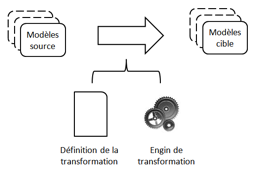
\includegraphics[width=0.7\textwidth]{Chapitre1/composanttransfo.png}
 \end{center}
 \caption{Composants d'une transformation de modèle}
 \label{fig:composantTransfo}
\end{figure}

\subsubsection{Usages de la transformation de modèles }
Les transformations de modèles sont au cœur d'une démarche dirigée par les 
modèles~:~elles permettent d'automatiser les manipulations subies par les 
modèles telles que la modification, la création, l'adaptation, la composition ou 
encore le filtrage de modèles, à travers la réutilisation systématique 
d'informations contenues dans les modèles existants. 

Il est possible de recourir aux transformations de modèles sur tout le cycle de 
vie d'un système. Les usages les plus répondus sont le raffinement, 
l'intégration d'outils, la composition, l'analyse, la simulation et 
l'optimisation que nous présentons dans la suite de ce document. 

\begin{description}

\item \textbf{Raffinement}

Le raffinement consiste à rajouter plus de détails au modèle initial. Ce type de 
transformation peut aussi bien être endogène (métamodèles source et cible 
identique) ou exogène (métamodèle source et cible différents). Le raffinement se 
prête parfaitement à toute la partie descendante du cycle en V où les modèles 
passent à des niveaux d'abstraction plus bas. Ceci revient à faire des 
transformations successives de type modèle-à-modèle et une transformation de 
type modèle-à-texte pour aboutir au code final.

Raffiner un modèle revient à décomposer des concepts de haut niveau, à choisir 
un algorithme particulier, à spécialiser un concept pour un contexte donné ou 
encore à le concrétiser sous forme d'une solution exécutable par une machine en 
générant le code à partir de modèles de plus haut niveau d'abstraction 
\cite{czarnecki2000intentional}. 

\item \textbf{Intégration d'outil}

Il existe une panoplie d'outils disponibles pour créer, manipuler, analyser ou 
encore simuler des modèles. Souvent ces outils utilisent des métamodèles 
internes et des espaces techniques qui leurs sont propres. Ainsi, l'échange de 
modèle entre ces outils est compromis et l'interopérabilité est fortement 
entravée. L'utilisateur se trouve obligé d'utiliser un seul et même outil sur 
tout le cycle de vie du système et ne peut donc pas tirer avantage des 
possibilités offertes par d'autres outils plus adaptés à ses besoins à certaines 
étapes.

L'intégration d'outil est une solution pour palier la divergence syntaxique et 
sémantique des outils et des langages de modélisation par le biais la 
transformation de modèle \cite{tratt2005model}. Ce type de transformation permet 
de naviguer entre deux métamodèles, de synchroniser des modèles qui évoluent 
séparément sur des outils distincts, de faire des mapping entre métamodèles pour 
maintenir la cohérence des modèles conformes à ces métamodèles. Il sera donc 
possible de faire appel à des outils mieux adaptés à chaque étape du cycle de 
vie.

\item \textbf{Composition}

Pour réduire la complexité inhérente à la modélisation et à l'analyse de grands 
systèmes, tels que les Smart Grids par exemple, il est possible d'adopter une 
approche par points de vue qui permet de séparer les préoccupations. Les modèles 
produits correspondent donc à ces différents points de vue qu'on peut ainsi 
valider séparément dans un premier temps. A l'issue de cette approche modulaire, 
on pourra composer ces modèles, c'est-à-dire les assembler, pour aboutir un 
modèle global du système.

Dans le cas le plus simple, les deux modèles à composer sont conformes à un même 
métamodèle. Cependant, il est aussi possible de composer deux modèles conformes 
à deux métamodèles différents. 

Les deux modèles à composer peuvent aussi présenter des concepts en commun. Deux 
techniques existent pour composer des modèles, que nous illustrons dans la 
figure \ref{fig:compoExemple}~:

\begin{bulletList}
\item La première technique consiste à les fusionner. Dans ce cas, le modèle 
final résultant de la composition doit contenir toutes les informations issues 
des modèles initiaux, sans duplication des informations communes 
\cite{bezivin2006canonical}.
\cite{fleurey2008generic} présente un framework générique capable de composer 
des modèles indépendamment de leurs langages de modélisation. L'approche 
consiste à identifier les éléments qui représentent le même concept dans les 
deux modèles à composer et à les fusionner dans un nouveau modèle qui représente 
une vue intégrée de ces concepts. Il est aussi possible de spécialiser le 
framework pour un métamodèle particulier mais qui reste conforme au MOF.

\item La deuxième technique consiste à les tisser. Dans ce cas, on crée des 
correspondances entre les éléments qui représentent un même concept. Un 
métamodèle générique est créé pour définir les correspondances qui sont donc 
modélisées dans le modèle final. On y retrouve donc les éléments en commun 
dupliqués mais liés par un lien de correspondance. 
\end{bulletList}

Il est à noter que le modèle issu du tissage de deux modèles $M_{A}$ et $M_{B}$ 
peut être utilisé comme modèle intermédiaire que l'on note $M_{T}$ pour la 
fusion de $M_{A}$ et $M_{B}$. Dans ce cas L'opération de fusion consiste à 
produire un modèle $M_{AB}$ en prenant comme entrée $M_{A}$, $M_{B}$ et $M_{T}$. 
Cette technique est notamment utilisée par \cite{del2007semi} pour la 
composition semi-automatique de modèles.

\begin{figure}[!htbp]
 \begin{center}
  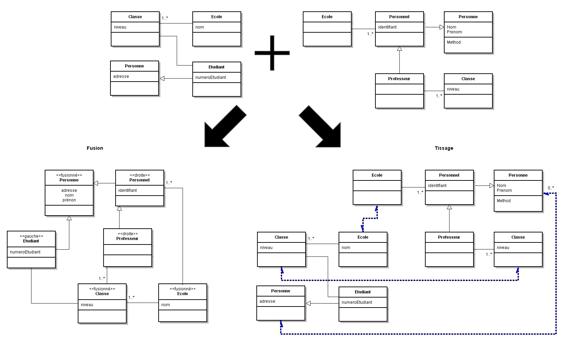
\includegraphics[width=1\textwidth]{Chapitre1/compoExemple.png}
 \end{center}
 \caption{Exemple de composition de deux modèles}
 \label{fig:compoExemple}
\end{figure}

\item \textbf{Simulation}

La transformation de modèle peut être utilisée pour simuler des modèles. En 
effet, une transformation de modèle peut mettre à jour le système modélisé. Dans 
ce cas, le modèle cible est une mise à jour du modèle source et la 
transformation est de type sur-place (modèles source et cible confondus). 

Par exemple, \cite{syriani2011multi} simule un comportement simple d'un jeu de 
Pacman en utilisant la transformation de modèle. La transformation spécifie les 
règles de transition qu'une instance du jeu peut prendre (Pacman et fantôme se 
trouvant dans la même case, Pacman et pomme se trouvant dans la même case, 
etc.). En ingénierie des langages, ceci revient à définir la sémantique 
opérationnelle d'un langage de modélisation. L'exécution de la transformation 
anime le modèle en fonction du comportement qu'on lui confère.

La transformation peut aussi être utilisée comme intermédiaire dans la 
simulation de modèle. Des modèles en entrée d'un outil de simulation externe 
sont produits par une transformation des modèles qu'on souhaite simuler. Cette 
technique permet de tirer profit d'outils de simulation existant sur le marché 
en utilisant l'intégration d'outils.

\item \textbf{Analyse et optimisation}

La transformation de modèle peut être utilisée pour les activités d'analyse de 
modèle. Une analyse simple telle que le calcul de métrique de similarité entre 
deux modèles via la transformation de modèle est donnée dans \cite{del2007semi} 
avec un modèle de transformation écrit en ATL \cite{jouault2006transforming}. 

Des analyses plus complexes sont possibles grâce à l'intégration d'outils 
d'analyse externes vers lesquels les modèles source sont transformés.

\cite{biehl2010integrating} propose d'utiliser la transformation de modèle pour 
l'analyse de sûreté de fonctionnement dans le domaine de l'automobile. Les 
modèles source sont transformés en modèles conformes au métamodèle de l'outil 
d'analyse de sûreté de fonctionnement retenu.
 
L'optimisation vise à améliorer les propriétés non fonctionnelles des modèles 
telle que l'évolutivité, la fiabilité, la modularité, etc. L'optimisation est 
typiquement utilisée sur les modèles d'architecture. Les transformations 
utilisées pour l'optimisation sont de types endogènes car on cherche à affiner 
la conception de modèles existants. La réingénierie est un exemple de 
transformation utilisée pour optimiser les modèles~:~on cherche à améliorer la 
maintenabilité, la lisibilité et l'évolutivité des modèles.

\end{description}

\subsubsection{Approches existantes pour la transformation de modèle}  
Le recours à la transformation de modèle est l'objet de recherches informatiques 
antérieures à l'apparition de l'approche IDM. Par exemple, les compilateurs 
utilisent la transformation pour passer du code source au fichier binaire 
\cite{aho1985compilers}. Ce type de transformation est restreint au domaine de 
la programmation informatique. La transformation de modèle embrasse un domaine 
plus large encore.

Nous trouvons dans la littérature plus d'une trentaine d'approches différentes 
de transformation de modèle \cite{syriani2011multi}. Czarnecki et Helsen 
proposent une classification de ces approches selon plusieurs critères tels que 
le paradigme retenu pour définir la transformation, la relation entre les 
modèles sources et cibles, la directivité de la transformation, le nombre de 
modèles cible et source, l'orchestration et l'ordonnancement des règles de 
transformation, etc. \cite{czarnecki2006feature}.

\cite{blanc2011mda} retient trois grandes catégories d'approches~:

\begin{bulletList}
\item Par programmation

Les modèles offrent une interface qui permet d'écrire les transformations dans 
un langage de programmation. Mais cette technique relève plus de la 
programmation que de la modélisation. Ce sont en fait des applications 
informatiques qui ont la particularité de manipuler des modèles. L'avantage de 
cette approche est que l'on utilise un langage de programmation généraliste tel 
que Java ou C++ pour écrire les transformations. Ainsi le programmeur n'a pas 
besoin d'apprendre un nouveau langage. Cependant ces applications ont tendance à 
devenir difficilement maintenables. 

\item Par template 

Dans cette approche on définit des canevas des modèles cibles. Ces modèles 
contiennent des paramètres qui seront remplacés par les informations contenues 
dans les modèles source. Ce type de transformation est souvent utilisé pour les 
transformations modèle-à-texte et est associé au visitor-pattern qui va 
traverser la structure interne du modèle source. Cette approche est utilisée par 
l'outil Enterprise Architect par exemple. 

\item Par modélisation

Cette approche vise à appliquer les principes de l'IDM aux transformations de 
modèles elles-mêmes. Ainsi, on produit des modèles de transformation prennes, 
réutilisables et indépendants des plates-formes d'exécution 
\cite{bezivin2006model}. 

Pour cela, on utilise des langages de modélisation dédiés à l'activité de 
transformation de modèles. Cette approche considère donc la transformation comme 
un modèle à part entière conforme à un métamodèle de transformation. La figure 
\ref{fig:TransfoPrincipe} , illustre cette approche en positionnant la 
transformation sur les différents niveaux d'abstraction de l'IDM. Elle corrobore 
ainsi la vision unificatrice de l'IDM à travers le paradigme du « tout est 
modèle » \cite{bezivin2005unification}. Le langage de transformation ATL, que 
nous présentons dans la section~\ref{sec:ATL}, a été développé dans ce sens. 

\end{bulletList}

\begin{figure}[!htbp]
 \begin{center}
  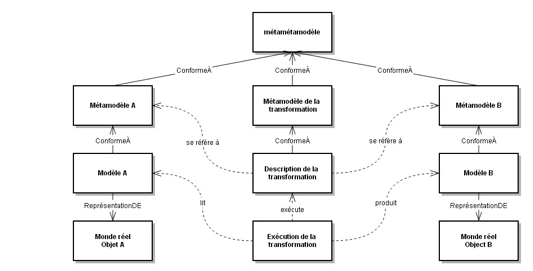
\includegraphics[width=1\textwidth]{Chapitre1/transfoPrincipe.png}
 \end{center}
 \caption{Méta niveaux d'une transformation de modèle}
 \label{fig:TransfoPrincipe}
\end{figure}

\subsection{Langages et outils pour la transformation de modèle}
Dans cette section, nous introduisons succinctement quelques langages et outils 
dédiés à la transformation de modèles, sans viser à l'exhaustivité.

\subsubsection{ATL}
\label{sec:ATL}
Atlas Transformation Language (ATL) \cite{jouault2006transforming} 
\cite{jouault2008atl} est né de la volonté de proposer des langages de 
modélisation dédiés à la transformation de modèle en définissant un métamodèle 
et des outils pour l'exécution des transformations. Il permet de réaliser des 
transformations de type modèle-à-modèle et de type modèle-à-texte.

ATL  est un langage hybride (déclaratif et impératif) à base de règles OCL (OMG 
2014). Une règle déclarative, appelée Matched rule, permet de décrire 
l'implémentation de mapping simples entre les modèles source et cible en 
utilisant des patrons source (\textit{InPattern}) mappés avec les éléments 
source et des patrons cibles (\textit{outPattern}) mappés avec les éléments 
cible. 

L'approche impérative explicite les étapes d'exécution de la transformation à 
travers les Helpers. Ce mécanisme de Helpers permet en outre d'éviter la 
redondance de code et la création de longues règles écrites en OCL, ce qui 
confère une meilleure lisibilité aux programmes ATL. 

Une transformation écrite en ATL est composée d'un ensemble de règles qui 
spécifient comment créer et initialiser les éléments des modèles cible. Il n'est 
pas possible de spécifier l'ordre d'exécution des règles de transformation. Cet 
ordre est établi automatiquement, exception faite pour les \textit{lazy rules} 
qui ont besoin qu'on fasse spécifiquement appel à elles. ATL est conforme au 
méta-métamodèle MOF et est doté d'une syntaxe concrète textuelle. Il est intégré 
à l'environnement Eclipse. Une transformation prend en entrée un ensemble de 
modèles conformes à Ecore (EMF 2014) ou KM3 \cite{jouault2006km3}.

ATL ne prend pas en charge les transformations incrémentales. Il commence par 
lire entièrement les modèles source et génère des modèles cible complet. Les 
modifications manuelles dans les modèles cible ne sont donc pas préservées si 
l'on opère une nouvelle transformation.

ATL peut réaliser des transformations sur  place, c'est-à-dire, une 
transformation où le modèle source et le modèle source sont confondus en 
utilisant le mode raffinement de modèle. Cependant ce mode présente quelques 
limitations avec certaines fonctionnalités comme celle des \textit{lazy rules}.

\subsubsection{QVT}
Le framework Query View Transformation (QVT) \cite{kurtev2008state} 
\cite{omg2011meta} a rejoint la batterie de standards de l'OMG. Le métamodèle de 
QVT est conforme au MOF. Comme ATL, QVT se base sur OCL pour accéder aux 
éléments des modèles.
QVT définit trois langages de transformation de type modèle-à-modèle. 
QVT-Relations (QVT-R) et QVT-Core (QVT-C) sont des langages déclaratifs qui 
adressent deux niveaux d'abstraction différents. QVT-Operational Mappings 
(QVT-OM) est un langage impératif qui étend QVT-R et QVT-C.

QVT-R est un langage de transformation de haut niveau d'abstraction doté de 
syntaxes concrètes textuelle et graphique. Les transformations, 
bidirectionnelles, sont spécifiées sous forme de relations entre les modèles 
source et cible. Une transformation a pour but de vérifier la cohérence entre 
deux modèles, renforcer la cohérence en modifiant le modèle cible, synchroniser 
deux modèles ou encore pour raffiner un modèle par une transformation sur-place. 
La sémantique de QVT-R est définie par une transformation vers QVT-C.

QVT-C est un langage de transformation de bas niveau qui sert de base pour 
QVT-R. Les deux ont le même niveau d'expressivité. Une transformation consiste 
en la déclaration de mapping entre les métamodèles source et cible en utilisant 
des patterns. Contrairement à QVT-R, la traçabilité est explicitement définie à 
travers les liens entre les métamodèles.

QVT-OM est un langage de transformation impératif qui étend QVT-R avec des 
constructions impératives basée sur une extension impérative de OCL. Les 
transformations sont unidirectionnelles mais établissent explicitement des 
modèles de traçabilité.

QVT est aussi doté d'un mécanisme de \textit{blackbox} qui permet de faire appel 
à des algorithmes complexes écrits dans n'importe quel langage de programmation 
et d'utiliser des librairies existantes. Mais ce mécanisme rend la 
transformation opaque puisqu'il n'est pas contrôlé par le moteur d'exécution. 
Nous pouvons citer SmartQVT ou encore ModelMorf comme machines d'exécution de 
transformation écrite en QVT.

\subsubsection{Kermeta}
Kermeta est un langage généraliste de méta-modélisation exécutable et de 
méta-programmation orientée objet qui peut aussi décrire des transformations de 
modèle. Intégré à EMF, il est doté d'un métamodèle conforme au MOF qu'il étend 
avec un langage d'action impératif utilisé pour écrire le corps des opérations 
définies sur les concepts d'une syntaxe abstraite (ce qui revient à doter une 
syntaxe abstraite d'une sémantique opérationnelle). On peut ainsi décrire 
n'importe quel traitement sur un modèle ce qui est assimilé à une transformation 
de modèle.

Le langage d'action de Kermeta permet d'écrire des expressions impératives qui 
spécifient explicitement la construction des éléments des modèles cible. A 
l'inverse de QVT-OM, Kermeta n'est pas un langage à base de règles.  
Kermeta est capable de gérer les exceptions mais les transformations 
multidirectionnelles ne sont pas supportées par les outils d'exécution. Il en 
est de même pour la transformation incrémentale. Les modèles source sont lus en 
une seule fois et les modèles cible sont produits complets lors de l'exécution 
de la transformation.






 




